\documentclass{article}
\usepackage[russian]{babel}
\usepackage[utf8]{inputenc}
\usepackage[T2]{fontenc}
\usepackage{graphicx}
\graphicspath{ {images/} }

\title{ТМП ДЗ №1}
\author{Максим Щемилкин A-05-19}
\date{30 марта 2022}

\begin{document}
\maketitle
\section{Построить конечный автомат, распознающий язык}


    \quad 1. $L = \{w \in \{a, b, c\}^*\quad|w|_c = 1\}$
    \begin{center}
        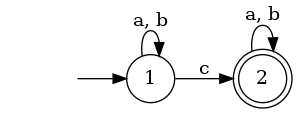
\includegraphics[width=0.4\textwidth]{pic1.dot}
    \end{center}
    \quad 2. $L = \{w \in \{a, b\}^* \quad |w|_a \leq 2, |w|_b \geq 2\}$
    \begin{center}
        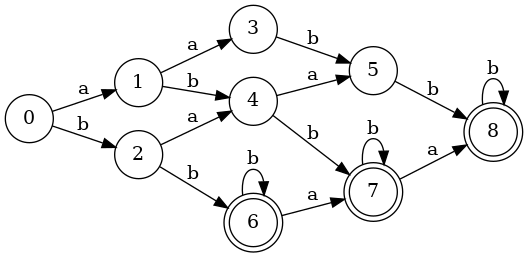
\includegraphics[width=0.8\textwidth]{pic2.dot}\\
    \end{center}
    Это решение получается через перебор первых 4 символов. Такой же результат можно получить через произведение двух грамматик:\\
    $$L_1 = \{w \in \{a, b\}^* \quad |w|_a \leq 2\}, \quad L_2 = \{w \in \{a, b\}^* \quad |w|_b \geq 2\}$$\\
    \begin{center}
        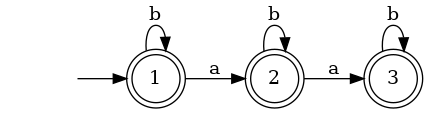
\includegraphics[width=0.45\textwidth]{pic3.dot}
        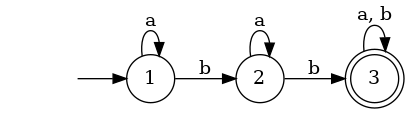
\includegraphics[width=0.45\textwidth]{pic4.dot}
    \end{center}
    \begin{center}
        \begin{tabular}{|c|c|c|}
            \hline
            Сочетания точек & По А & По В \\
            \hline
            11 & 21 & 12\\
            12 & 22 & 13\\
            13 & 23 & 13\\
            21 & 31 & 22\\
            22 & 32 & 23\\
            23 & 33 & 23\\
            31 &  & 32\\
            32 &  & 33\\
            33 &  & 33\\
            \hline
        \end{tabular}\\
    \end{center}
    Получим:
    \begin{center}
        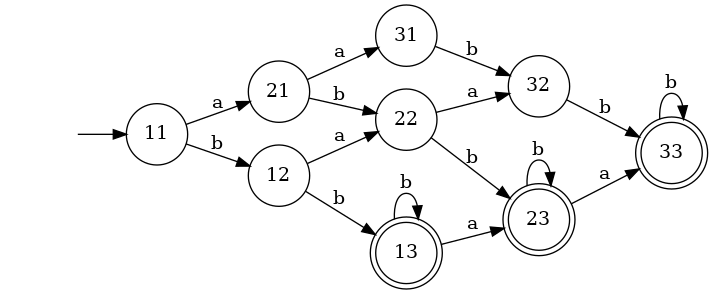
\includegraphics[width=0.9\textwidth]{pic5.dot}\\
    \end{center}
    \quad 3. $L = \{w \in \{a, b\}^* \quad |w|_a \neq |w|_b\}$
    \begin{center}
        Нет такого конечного автомата
    \end{center}
    \quad 4. $L = \{w \in \{a, b\}^* \quad ww = www\}$\\
    Это возможно только для языка, состоящего из пустого слова, так как при $|w|>0 ww \neq www$. Можем построить недерминированный КА:
    \begin{center}
        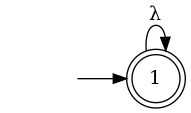
\includegraphics[width=0.3\textwidth]{pic6.dot}\\
    \end{center}
    
\section{Построить КА, используя прямое произведение}

    1. $L_1 = \{w \in \{a, b\}^* \quad |w|_a \geq 2 \wedge |w|_b \geq 2\}$\\
    Разобьем на 2 автомата:
    $$L_11 = \{w \in \{a, b\}^* \quad |w|_a \geq 2\}, \quad L_12 = \{w \in \{a, b\}^* \quad |w|_b \geq 2\}$$\\
    \begin{center}
        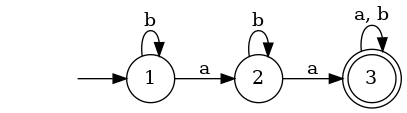
\includegraphics[width=0.45\textwidth]{pic7.dot}
        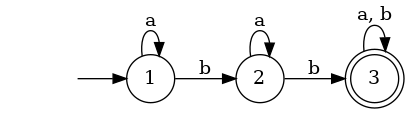
\includegraphics[width=0.45\textwidth]{pic4.dot}
    \end{center}
    Значит, $L = L_11 \wedge L_12$. Имеем $\Sigma = {a, b}, s = 11, T = 33$. Зафиксируем переходы между новыми вершинами:
    \begin{center}
        \begin{tabular}{|c|c|c|}
            \hline
            Сочетания точек & По А & По В \\
            \hline
            11 & 21 & 12\\
            12 & 22 & 13\\
            13 & 23 & 13\\
            21 & 31 & 22\\
            22 & 32 & 23\\
            23 & 33 & 23\\
            31 & 31 & 32\\
            32 & 32 & 33\\
            33 & 33 & 33\\
            \hline
        \end{tabular}\\
    \end{center}
    Получим:
    \begin{center}
        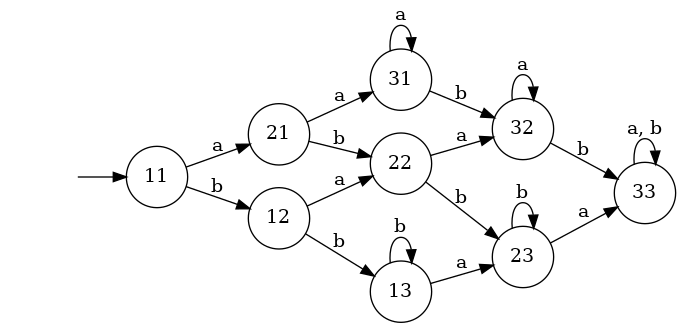
\includegraphics[width=0.9\textwidth]{pic8.dot}\\
    \end{center}
    
    2. $L_2 = \{w \in \{a, b\}^* \quad |w| \geq 3 \wedge |w|\quad odd\}$\\
    Разобьем на 2 автомата:
    $$L_21 = \{w \in \{a, b\}^* \quad |w| \geq 3\}, \quad L_22 = \{w \in \{a, b\}^* \quad |w|\quad odd\}$$
    \begin{center}
        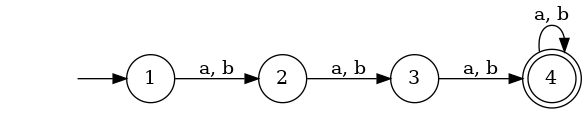
\includegraphics[width=0.6\textwidth]{pic9.dot}
        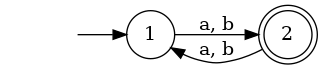
\includegraphics[width=0.3\textwidth]{pic10.dot}
    \end{center}
    Значит, $L = L_21 \wedge L_22$. Имеем $\Sigma = {a, b}, s = 11, T = 42$. Зафиксируем переходы между новыми вершинами:
    \begin{center}
        \begin{tabular}{|c|c|c|}
            \hline
            Сочетания точек & По А & По В \\
            \hline
            11 & 22 & 22\\
            12 & 21 & 21\\
            21 & 32 & 32\\
            22 & 31 & 31\\
            31 & 42 & 42\\
            32 & 41 & 41\\
            41 & 42 & 42\\
            42 & 41 & 41\\
            \hline
        \end{tabular}\\
    \end{center}
    Получим:
    \begin{center}
        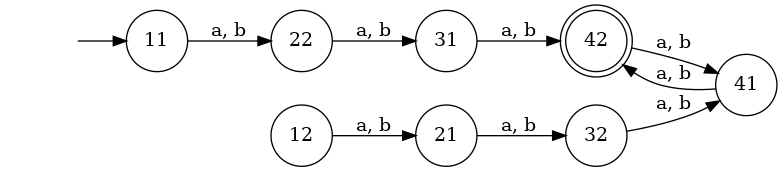
\includegraphics[width=0.9\textwidth]{pic11.dot}\\
    \end{center}
    Так как в вершину 12 попасть нельзя, можно автомат немного упростить:
    \begin{center}
        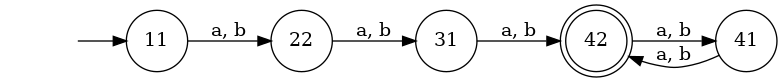
\includegraphics[width=0.9\textwidth]{pic12.dot}\\
    \end{center}
    
    3. $L_3 = \{w \in \{a, b\}^* \quad |w|_a\, \vdots\, 2 \wedge |w|_b\, \vdots\, 3\}$\\
    Разобьем на 2 автомата:
    $$L_31 = \{w \in \{a, b\}^* \quad |w|_a\, \vdots\, 2\}, \quad L_32 = \{w \in \{a, b\}^* \quad |w|_b\, \vdots\, 3\}$$
    \begin{center}
        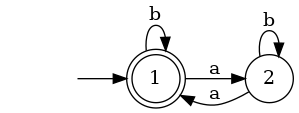
\includegraphics[width=0.4\textwidth]{pic13.dot}
        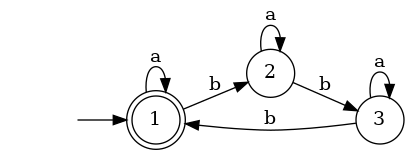
\includegraphics[width=0.5\textwidth]{pic14.dot}
    \end{center}
    Значит, $L = L_31 \wedge L_32$. Имеем $\Sigma = {a, b}, s = 11, T = 11$. Зафиксируем переходы между новыми вершинами:
    \begin{center}
        \begin{tabular}{|c|c|c|}
            \hline
            Сочетания точек & По А & По В \\
            \hline
            11 & 21 & 12\\
            12 & 22 & 13\\
            13 & 23 & 11\\
            21 & 11 & 22\\
            22 & 12 & 23\\
            23 & 13 & 21\\
            \hline
        \end{tabular}\\
    \end{center}
    Получим:
    \begin{center}
        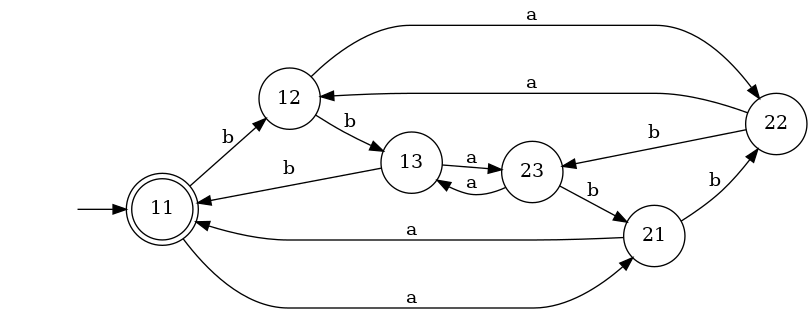
\includegraphics[width=0.9\textwidth]{pic15.dot}
    \end{center}
    
    
    4. $L_4 = \overline{L_3}$\\
    Чтобы построить отрицание, нужно обратить конечные вершины, то есть получим:
    \begin{center}
        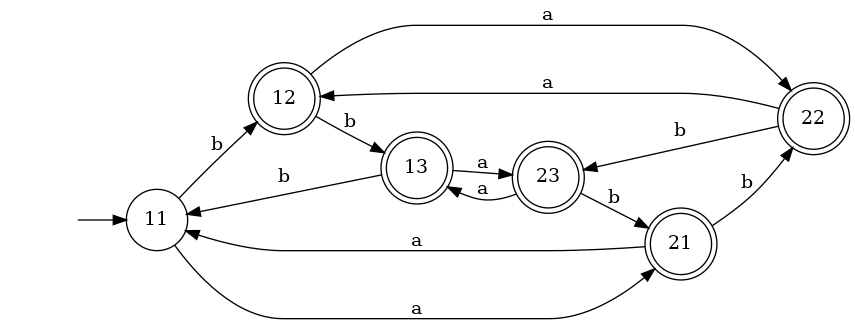
\includegraphics[width=0.9\textwidth]{pic16.dot}
    \end{center}
    
    5. $L_5 = L_2 \setminus L_3 = L_2 \wedge L_4 $\\
    Найдём пересечение двух языков:
    \begin{center}
        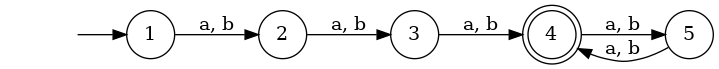
\includegraphics[width=0.9\textwidth]{pic2_5_1.dot}
        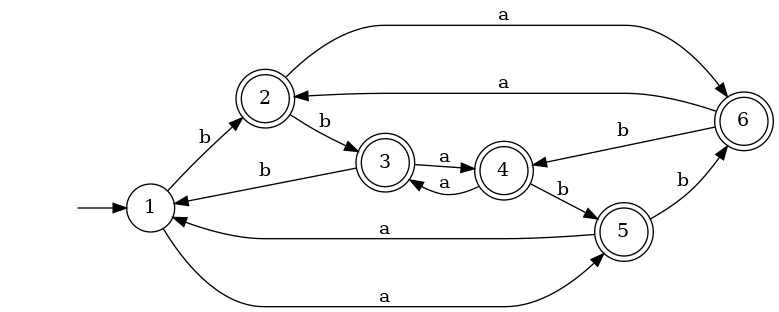
\includegraphics[width=0.9\textwidth]{pic2_5_2.dot}
    \end{center}
    $L_5 = L_2 \wedge L_4$. Имеем $\Sigma = \{a, b\}, s = 11, T = 42$. Зафиксируем переходы между новыми вершинами:
    \begin{center}
        \begin{tabular}{|c|c|c|}
            \hline
            Сочетания точек & По А & По В \\
            \hline
            11 & 25 & 22\\
            12 & 26 & 23\\
            13 & 24 & 21\\
            14 & 23 & 25\\
            15 & 21 & 26\\
            16 & 22 & 24\\
            21 & 35 & 32\\
            22 & 36 & 33\\
            23 & 34 & 31\\
            24 & 33 & 35\\
            25 & 31 & 36\\
            26 & 32 & 34\\
            31 & 45 & 42\\
            32 & 46 & 43\\
            33 & 44 & 41\\
            34 & 43 & 45\\
            35 & 41 & 46\\
            36 & 42 & 44\\
            41 & 55 & 52\\
            42 & 56 & 53\\
            43 & 54 & 51\\
            44 & 53 & 55\\
            45 & 51 & 56\\
            46 & 52 & 54\\
            51 & 45 & 62\\
            52 & 46 & 43\\
            53 & 44 & 41\\
            54 & 43 & 45\\
            55 & 41 & 46\\
            56 & 42 & 44\\
            \hline
        \end{tabular}\\
    \end{center}
    Получим:
    \begin{center}
        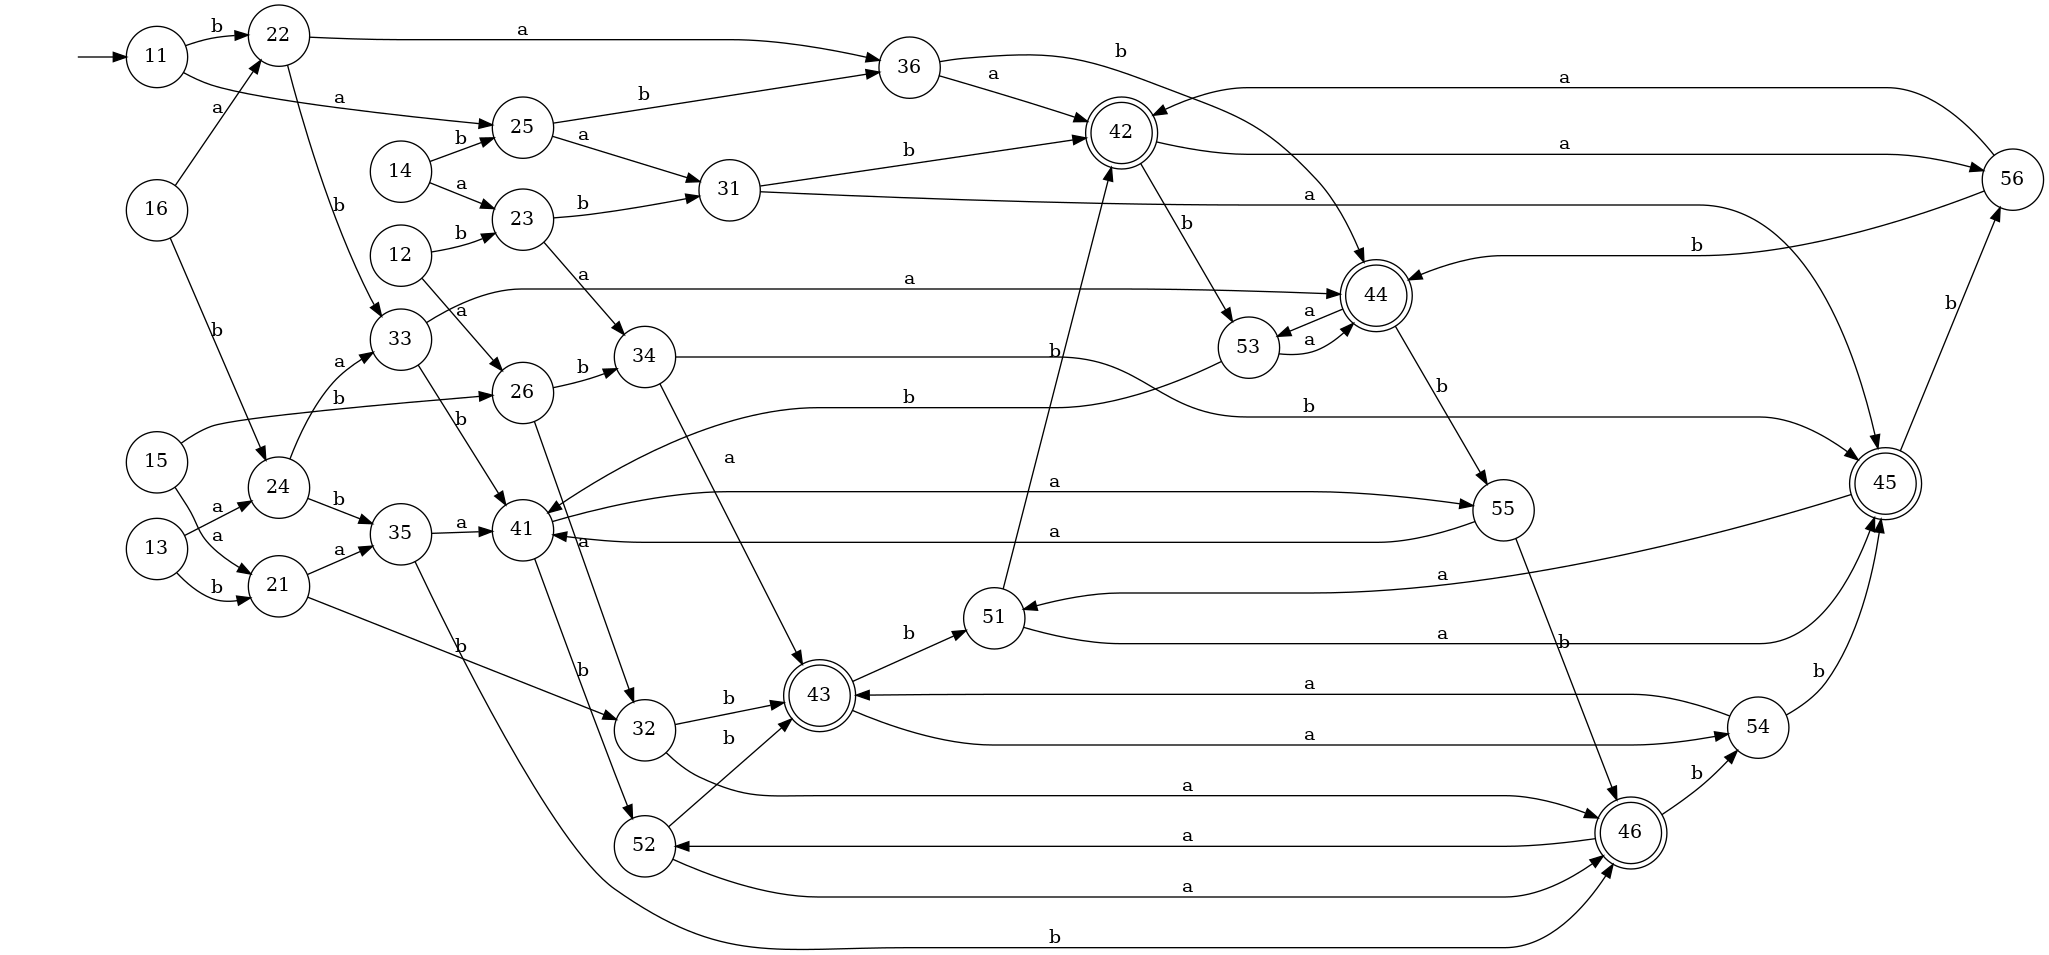
\includegraphics[width=1\textwidth]{pic2_5_3.dot}\\
    \end{center}
    
\section{Построить минимальный ДКА по регулярному выражению}
    1. $(ab+aba)^*a$\\
    Недетерминированный КА по данному выражению:
    \begin{center}
        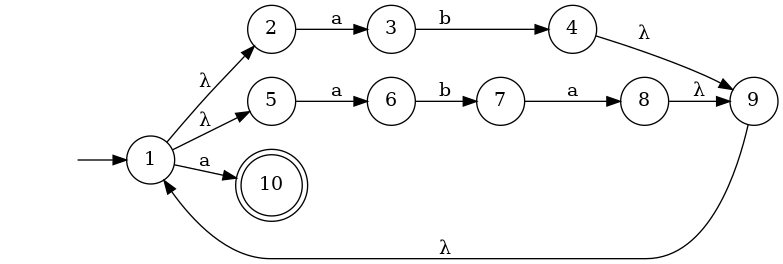
\includegraphics[width=1\textwidth]{pic3_1_1.dot}\\
    \end{center}
    \begin{center}
        \begin{tabular}{|c|c|c|}
            \hline
            Сочетания точек & По А & По В \\
            \hline
            1 & 3 6 10 & \\
            3 6 10 & & 4 7 \\
            4 7 & 8 3 6 10 & \\
            8 3 6 10 & 3 6 10 & 4 7\\
            \hline
        \end{tabular}\\
    \end{center}
    Теперь можем нарисовать ДКА:
    \begin{center}
        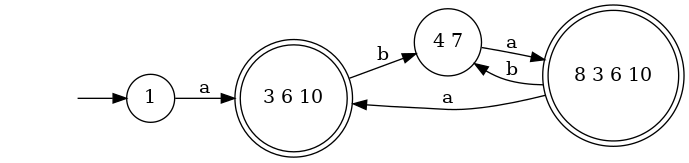
\includegraphics[width=1\textwidth]{pic3_1_2.dot}\\
    \end{center}
\end{document}
